%%%%%%%%%%%%%%%%%%%%%%%%%%%%
%\subsection{Validation of Calibration Hardware Systems}

All calibration designs presented in the previous section require full system validation before being deployed in the \dword{dune} \dword{fd}. 

Although laser calibration systems are being operated in other \dword{lartpc} experiments (e.g., \dword{microboone}, future \dword{sbnd} runs), they have stringent requirements in terms of mechanical and optical precision , long-term reliability, laser track length, performance of the \dword{lbls}, \dword{daq} interface, and effect on \efield, especially due to the location of the periscope in the gap between the \dword{fc} and \dword{crp}. All of these lead to corresponding goals for a test installation and operation in \dword{pddp} that could be done in the post-LS2 run. 

We are currently considering available suitable ports in \dword{pddp} that can be used for these tests.
As Figure~\ref{fig:protoDUNEDP_topView_marked} shows, \dword{pddp} has ports the same size as the \dword{dune} \dword{fd} that could, in principle, be used for these tests.  If a pair of ports can be used, then one could even have crossing tracks within a single drift volume. However, the available ports are outside the \dword{tpc}, so coverage will be limited by shadowing from the \dword{fc}, and no reflector panels should be installed close to the laser periscopes.

\begin{dunefigure}[Top view of the \dword{pddp} cryostat showing various penetrations]{fig:protoDUNEDP_topView_marked}
{Top view of the \dword{pddp} cryostat showing various penetrations. Ports shown in red are marked as spares and, pending verification, could be used to test the calibration systems. These are the same diameter (\SI{250}{\milli\m} outer diameter) as the calibration ports of the \dword{dune} \dword{fd} and are located outside the \dword{tpc}. The largest port at the right side of the cryostat is a human access port.}
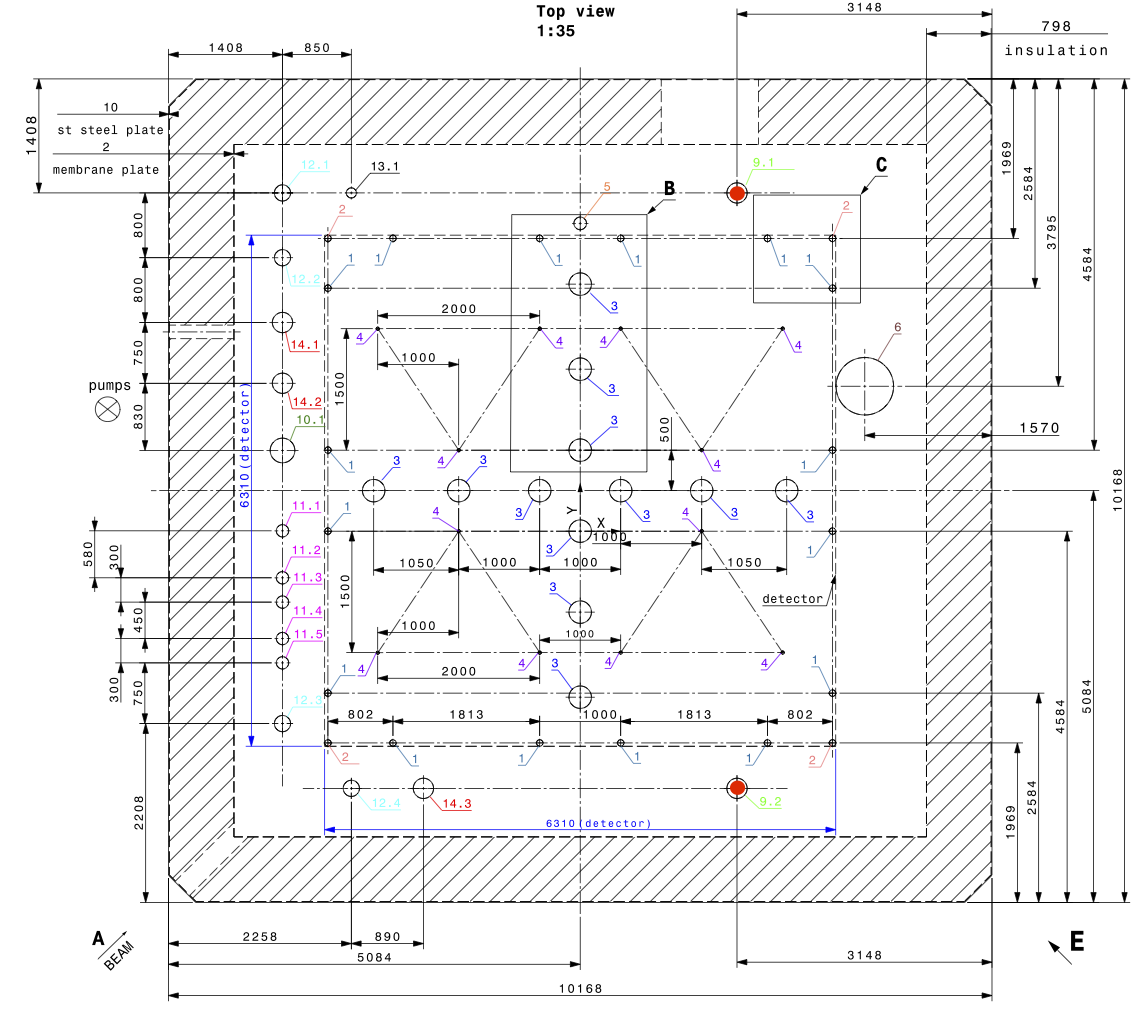
\includegraphics[height=4.0in]{protoDUNEDP_topView_marked.png}
\end{dunefigure}

The goal of validation would be to test all aspects of the system design, installation, alignment, operation, interfaces with \dword{daq}, and analysis, among others. \dword{pddp}, because it is located at the surface, could measure the \efield map with cosmics to compare with the one from the laser system to improve the analysis methods or identify weak points in the design. 
%An important design parameter is the length of a laser track. Our design assumes that \SI{12}{\m} is possible; \dword{microboone} has demonstrated only up to \SI{10}{\m}, but the track could be longer, depending on laser intensity. Measurements are limited by the size of the detector, but one way to gain information on longer tracks would be to make a scan with low laser intensities, so the end of the track would be visible and register how the maximum obtained track length scales with intensity. An extrapolation to the \dword{dune} \dword{fd} laser intensity would tell us the maximum length possible. Such a measurement could also be done at \dword{microboone}, \dword{sbnd}.

%\todo{SG: Jose, we had this paragraph on lifetime in SP, modify this for DP? it says APA in one sentence.}
An important aspect of the development plan, to be carried out at \dword{pddp}, is the characterization of the charge created by the laser beam ionization as a function of distance travelled in the \dword{lar} and the laser beam intensity. This dependence is thought to be affected by self-focusing effects due to the high light intensity, but it can be studied by measuring the collected charge distribution from a series of tracks close, and parallel, to the \dwords{crp} in order to break any correlations with the electron lifetime. This measured charge function could then be used with tracks in different directions to obtain a measurement of electron lifetime, which would significantly increase the capabilities of the laser system.  

The pulsed neutron source is a new idea never used in other experiments, so a \dword{pddp} test is essential. The corner human access ports similar to the ones in the \dword{dune} \dword{fd} could be used for this test.
%The post-beam run being proposed for ProtoDUNE-SP offers the opportunity to test the full system (DD Generator, Moderator, Transport Model, Data Analysis) in a definitive way before investing in the full PNS calibration for DUNE. The PNS group proposes to make such a run as soon as resources can be identified (independent of the other measurements above), starting with a commitment of engineering resources at CERN required to complete the necessary radiation safety shield design, and the mechanical design necessary to support the DD Generator and Moderator. The system used for ProtoDUNE-SP could also be used for ProtoDUNE-DP, and later installed in the DUNE detector. 

%For the radioactive source system, the cosmic induced background rate is too high at the surface to detect responses to the \dword{dune} gamma source; a higher intensity source could be deployed to test the detector response and analysis method. However, tests of functionality,  reliability, and safety of the mechanical deployment system are needed to show the source can be deployed and retrieved with no issues.

In addition to dedicated hardware validation runs at \dword{pddp}, other \dword{lar} experiments provide ample opportunities to develop and validate calibration tools and techniques, especially those relevant to the hardware being deployed. For example, the \dword{microboone} experiment is currently leading the development of analysis methods using laser data to extract an \efield map. Energy calibration techniques and related software tools are also being developed at various experiments (\dword{microboone}, ICARUS, \dword{lariat}, \dword{protodune}) that involve estimating and propagating uncertainties like \efield distortions, recombination, and other effects into physics signals. Other calibration related developments include \dword{daq} and calibration database design, all of which are being improved at \dword{sbn} and \dword{protodune}.
 
%%%%%%%%%%%%%%%%%%%%%%%%%%%%
%\subsubsection{Validation in Other Experiments}
%\label{sec:sp-calib-val-other}

%\cleardoublepage